\begin{frame}{Algorithmenanalyse}
	\textbf{O-Kalkül} \\
	{
		\renewcommand{\arraystretch}{2}%
	
		\begin{center}
			\begin{tabular}{ | c | c | c | }
				\hline
				$     o (f(n))$ & $<$ & echt schwächer wachsende Funktionen
				\\ \hline
				$     O (f(n))$ & $\leq$ & schwächer oder gleich stark wachsende Funktionen
				\\ \hline
				$\Theta (f(n))$ & $=$ & genau gleich stark wachsende Funktionen
				\\ \hline
				$\Omega (f(n))$ & $\geq$ & stärker oder gleich stark wachsende Funktionen
				\\ \hline
				$\omega (f(n))$ & $>$ & echt stärker wachsende Funktionen
				\\ \hline
			\end{tabular}
		\end{center}
	}
\end{frame}

\begin{frame}{Algorithmenanalyse}
	\textbf{O-Kalkül: Formeln} \\
	{
		\renewcommand{\arraystretch}{2}%
		\begin{center}
			\begin{tabular}{ | c | c | >{\quad}c<{\quad} | }
				\hline
				$f(n) \in o      (g(n))$ & $\Gdw$ & \(\lim\limits_{n \to \infty} \frac{f(n)}{g(n)} = 0\) 
				\\  \hline
				$f(n) \in O      (g(n))$ & $\Gdw$ & \(0 \leq \limsup\limits_{n \to \infty} \frac{f(n)}{g(n)} = c < \infty\)
				\\ \hline
				$f(n) \in \Theta (g(n))$ & \cellcolor{adaptingred} {\textbf{!} $\bm{\impliedby}$ \textbf{!}} & \(0 < \lim\limits_{n \to \infty} \frac{f(n)}{g(n)} = c < \infty\)
				\\ \hline
				$f(n) \in \Omega (g(n))$ & $\Gdw$ & \(0 < \liminf\limits_{n \to \infty} \frac{f(n)}{g(n)} = c \leq \infty\)
				\\ \hline
				$f(n) \in \omega (g(n))$ & $\Gdw$ & \(\limsup\limits_{n \to \infty} \frac{f(n)}{g(n)} = \infty\)
				\\ \hline
			\end{tabular}
			%\renewcommand{\arraystretch}{\stdarraystretch}
		\end{center}
	}
\end{frame}

\begin{frame}{Algorithmenanalyse}
	\textbf{Korrektheitsbeweis} \\
	
	\begin{itemize}
		\item Korrektheitsbeweis ist \textbf{zweiteilig}:
		
		\begin{itemize}
			\item 1. Teil -- \textbf{Funktionalität}: Mit Invariante beweisen, dass der Algorithmus ein \textbf{korrektes} Ergebnis erzeugt
			
			\item 2. Teil -- \textbf{Terminierung}: Beweisen (ggf. anhand einer Invariante), dass der Algorithmus „irgendwann \textbf{fertig} wird“.
		\end{itemize}
		
		\item \textbf{Aufgabenstellung beachten}: Wenn („nur“) eine Invariante angegeben/bewiesen werden soll \impl Terminierungsbeweis nicht nötig!
	\end{itemize}
\end{frame}

\begin{frame}{Algorithmenanalyse}
	\textbf{Invarianten} \\
	
	\begin{itemize}
		\item Invariante finden: Manchmal offensichtlich, manchmal \textbf{Kreativität} gefragt
		
		\item Invarianten beweisen – im Prinzip \textbf{Induktion}:
		
		\item „IA“: Invariante gilt bei \textbf{Beginn} des Algorithmus / der Schleife
		
		\item „IV“: Die Invariante war beim Ende des \textbf{vorherigen} Ausführungsschrittes gültig
		
		\item „IS“: Mithilfe der IV zeigen, dass die Invariante auch beim Ende des \textbf{aktuellen} Ausführungsschrittes gültig ist
		\item \textbf{Achtung}: Invarianten müssen auch \textbf{nach Ende der Schleife} noch gelten!
	\end{itemize}
\end{frame}

\begin{frame}{Algorithmenanalyse}
	\textbf{Beispiele für Invarianten} \\
	\begin{itemize}
		\item \textbf{Binäre Suche}: Gesuchtes Element kann \textbf{nicht} im ignorierten Bereich liegen
		\item \textbf{Quicksort}: Links $\leq pivot < $ Rechts
		\item \textbf{Mergesort}: Listen, die von rekursiven Aufrufen zurückgegeben werden, sind \textbf{sortiert}
		\item \textbf{Dijkstra}: Endgültiger kürzester Pfad zum $min$ der $PriorityQueue$ ist bekannt
		\item Doppelt verkettete \textbf{Liste}: $next \access prev = prev \access next = \KwThis$
	\end{itemize}
\end{frame}

\begin{frame}{Algorithmenanalyse}
	\underline{Aufgabe: Korrektheitsbeweis} \\
	Beweist die Korrektheit von $ArraySum$: 
	\begin{algorithm}[H]
		\Function{ArraySum$(A: \KwArray[1..n] \KwOf \R): \R$}{
			$i := 1$ \;
			$s := 0$ \;
			\While{$i \leq n$}{
				$\KwInvariant \only<1|handout:0>{???}\visible<2>{1 \leq i \leq n+1 \KwAnd s = \sum\limits_{j=1}^{i-1} A[j]}$ \;
				$s := s + A[i]$ \;
				$i\pp$ \;	
			}
			\Return{$s$}
		}
	\end{algorithm}
\end{frame}

\newcommand{\selsortinvariant}{A[1\ ... \ i-1] \KwIs \text{sorted} \KwAnd \max(A[1\ ...\ i-1]) \leq \min(A[i..n])}
\begin{frame}{Beispiel SelectionSort}
	\begin{exampleblock}{SelectionSort}
		\begin{algorithm}[H]
			\small
			\Procedure{SelectionSort$(A: \KwArray[1..n] \KwOf Element)$}{
				\For{$i := 1 \KwTo n$}{
					\only<2>{$\KwInvariant \selsortinvariant $\;}
					minIndex $ := i$ \;
					\For{$j := i + 1 \KwTo n$}{
						\If{$A[j] < A[$minIndex$]$}{
							minIndex $ := j$ \;	
						} 
					} 	
					$\KwAssert A[minIndex] = \min(A[i..n])$ \;
					$swap(A[i], A[minIndex])$ \;
				}	
			}
		\end{algorithm}
	\end{exampleblock}
\end{frame}

\begin{frame}{SelectionSort -- Beweis Invariante}
	\begin{overlayarea}{\textwidth}{.60\textwidth}
		{Definiere \quad $\max(()) := -\infty$ \quad und \quad $\min(()) := +\infty$. \\} 
		
		Beweis Invariante: \\ 
		$\quad\quad \selsortinvariant$ 
		
		{\hanging\textbf{IA}. ($i=1$): \ $A[1..0] = ()$ ist sortiert und $-\infty = \max(A[1..0]) \leq \min(A[1..n])$. \\}
		{\hanging\textbf{IV}. \textit{($i > 1$)}: \ Die Invariante galt am Ende des Durchlaufs $i - 1$. \\}
		\hanging\textbf{IS}. ($i - 1 \rightsquigarrow i$): \ Laut IV ist $A[1\ ...\ i-1]$ sortiert und \newline
		$\max(A[1\ ...\ i-1]) \leq \min(A[i...n])$ \quad und \quad $minIndex \in \{i,...,n\}$ \newline
		$\Rightarrow A[i-1] \leq A[minIndex]$ \ und \ $A[minIndex] \leq A[i]$. \newline
		$\Rightarrow A[minIndex]$ kann zur Fortsetzung der Sortierung problemlos nach $A[i]$ verschoben werden! 
		Tauschen von $A[i]$, $A[minIndex]$: \newline
		$\Rightarrow A[1..i]$ ist sortiert, \newline
		$A[i] = \max(A[1..i]) \leq \min(A[i+1 \ ... \ n]). \qed$ \newline
		
		$\Rightarrow$ Nach dem $n$-ten Schleifendurchlauf gilt also: $A[1..n]$ ist sortiert.
	\end{overlayarea}
\end{frame}

\begin{frame}{SelectionSort -- Beweis Terminierung}
	In diesem Fall trivial: 
	\begin{itemize}
		\item Schleifenvariable $i$ nach oben durch $n$ beschränkt
		\item ...und wird in jedem Durchlauf inkrementiert (und sonst nicht verändert)
		\implitem SelectionSort terminiert
	\end{itemize}
	\impl SelectionSort funktioniert! Yay! :D
\end{frame}






\begin{frame}{Das Master-Theorem (einfache Form)}
	$a, \textcolor{blue}{b}, c, \textcolor{darkgreen}{d}$ positive Konstanten und für $n \in \mathbb{N}$ sei 
	\[
	T(n) = 
	\begin{cases}
	a,  & \text{für } n = 1 \\
	\textcolor{darkgreen}{d} \cdot T(\lceil \frac{n}{\textcolor{blue}{b}} \rceil) + cn, & \text{für } n > 1
	\end{cases}.
	\]
	Dann gilt:
	\[
	T(n) \in 
	\begin{cases}
	\Theta(n),                                                        & \textcolor{darkgreen}{d} < \textcolor{blue}{b} \\
	\Theta(n \log n),                                                 & \textcolor{darkgreen}{d} = \textcolor{blue}{b} \\
	\Theta(n^{\log _{\textcolor{blue}{b}} \textcolor{darkgreen}{d}}), & \textcolor{darkgreen}{d} > \textcolor{blue}{b}
	\end{cases}.
	\] 
\end{frame}





\begin{frame}{Amortisierte Analyse}
	\textbf{How to} \\
	\begin{itemize}
		\item \textbf{Aggregatmethode}: Schätze nach oben ab: \\
		\qquad $
		\text{Gesamtkosten von $n$ \textcolor{blue}{beliebigen} Ops} = \text{„}T_\text{Gesamt}\text{“} \ \leq \ c \cdot n 
		$ \\
		($c$ irgendeine Konstante). \\ 
		Knifflig: Diese Abschätzung finden und zeigen. 
		\item \textbf{Kontomethode}: Zahle für jede Operation eine \textbf{konstante} Menge $c$ an Münzen aufs Konto ein. Zeige: Bei \textbf{nicht-konstanten} Operationen mit Kosten $k$ müssen \textbf{mindestens} $k$ Münzen aufm Konto sein.
		(Knifflig: Begründung und geeignetes $c$ finden)
		\item \textbf{Generell}: Genau überlegen, unter welchen Vorbedingungen die teuren Operationen auftreten
		\item \textbf{Aufgabenstellung} beachten, ob spezifische Methode gefordert ist! (Falls nein \impl klare logische Begründung des Sachverhaltes reicht (im Prinzip))
	\end{itemize}
	{\small Aufgabe: SS~2016 Blatt~3 A4 „Weltherrschaftskonferenz“}
\end{frame}




\begin{frame}{Listen und Co.}
	\textbf{Doppelt verkettete Liste} \\[0,125cm]
	\begin{itemize}
		\item Invariante: $next \access prev = prev \access next = \KwThis$
		\item \textbf{Dummy-Header} $h$ für Bequemlichkeit und als Sentinel (Wächter-Element) beim Suchen
		\item[\Pros] Flexibel
		\item[\Cons] Nicht cachefreundlich
	\end{itemize}
	\textbf{Unbeschränktes Array} \\[0,125cm]
	\begin{itemize}
		\item Array voll \impl Ziehe in \textbf{doppelt} so großes Array um
		\item Array viertel-voll 
		\impl Ziehe in \textbf{halb} so großes Array um
		\item[\Pros] Cachefreundlich
		\item[\Cons] Eher unflexibel
	\end{itemize}
\end{frame}

\begin{frame}{Listen und Co.}
	\textbf{Listen vs. Arrays}
	\begin{figure}[htp]
		\centering
		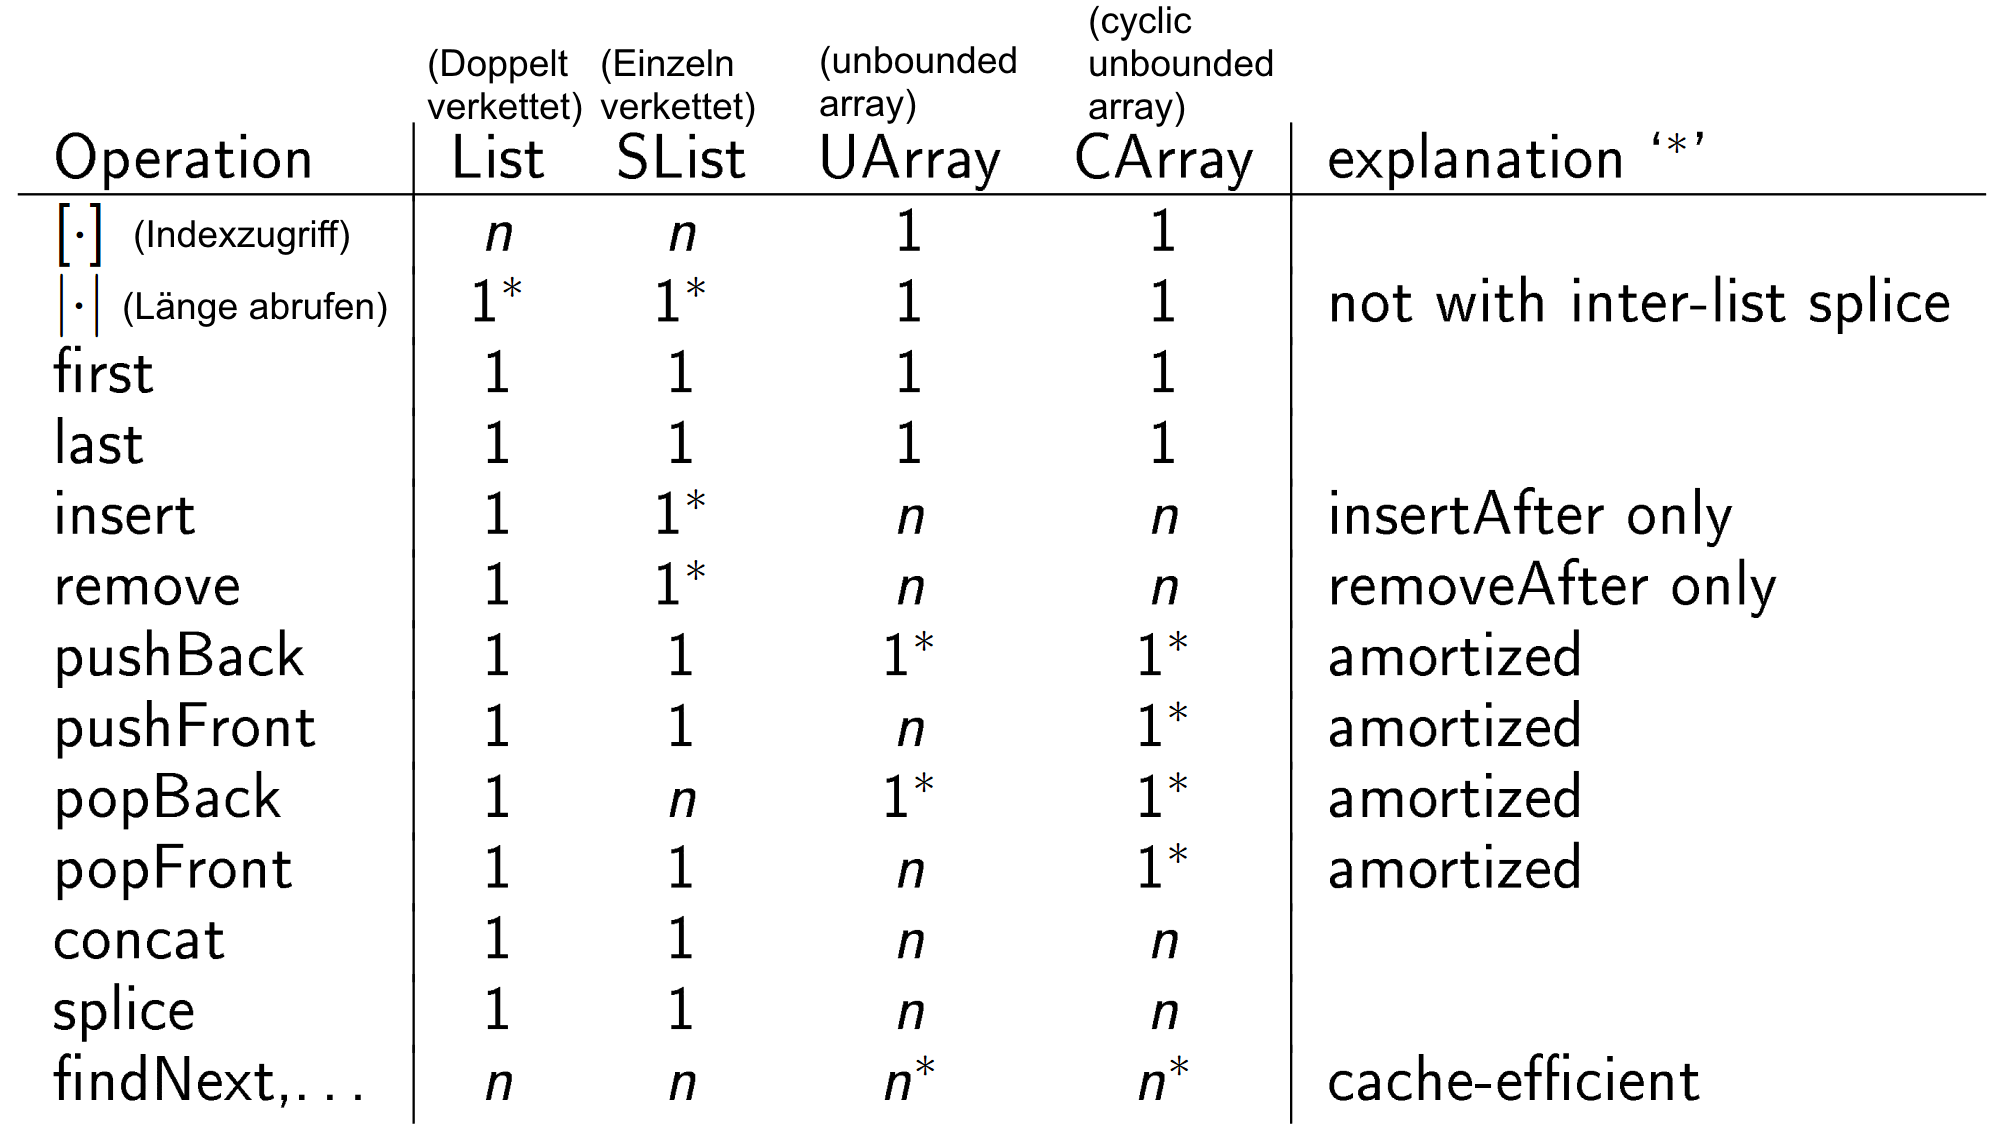
\includegraphics[height=6cm]{listenvsarrays}
	\end{figure}
\end{frame}

\begin{frame}{Listen und Co.}
	\underline{Aufgabe} \\
	Entwerft einen Stack, der $push$, $pop$ und $min$ kann und zwar in $O(1)$ (nicht amortisiert).
\end{frame}

\begin{frame}{Listen und Co.}
	\underline{Lösung} \\
	\begin{algorithm}[H]
		$BasicStack, MinimumStack: Stack$ \;
		\;
		\Function{min}{
			\Return{$MinimumStack$.getTop} \;
		}
		\;
		\Procedure{push$(e)$}{
			$BasicStack$.push$(e)$ \;
			\lIf{$e \leq \text{min}$}{$MinimumStack$.push$(e)$}	
		}
		\;
		\Function{pop}{
			$r := BasicStack$.pop$()$ \;
			\lIf{$r = \text{min}$}{$MinimumStack$.pop$()$}	
			\Return{$r$}
		}
	\end{algorithm}
\end{frame}




\begin{frame}{Hashing}
	\begin{itemize}
		\item \textbf{Erwartete} Laufzeit!
		\item \textbf{Hashfunktion} $h$ weist Elemente einem Platz zu 
		\item \textbf{Universelle} Hashfunktionen \quad --- \quad  Vorlesung: \\
		Wenn $n \in O(m)$ Elemente in die Hashtable eingefügt werden \impl erwartete $\abs{\text{Kollisionen}} \in O(1)$ 
		\item Typische univ. Hashfunktion: \\
		$h_a(x) := a \cdot x \mod m \quad (0 < a < m)$ \quad ($m$ \textbf{prim}!)
		\item Oder generisch (z. B., falls in Klausur nötig): „Sei $h$ eine beliebige Hashfunktion aus der Familie universeller Hashfunktionen“
	\end{itemize}
\end{frame}	

\begin{frame}{Hashing}	
	\textbf{Hashing mit verketteten Listen}
	\begin{itemize}
		\implitem Halte $\KwArrayOf \text{Lists}$: \\ 
		Werfe Element in die Liste, suche es dort
	\end{itemize}
	\pause
	\textbf{Hashing mit linearer Suche}
	\begin{itemize}
		\implitem Nur $\KwArrayOf \text{Element}$: \\
		Platz besetzt? Gucke rechts davon. \\
		Beim \textbf{Löschen}: Ggfs. wieder nach links zurückschieben!
		\item Ganz rechts im Array Platz dicht? \\
		\impl Pufferbereich (der dann hoffentlich langt)  \quad oder \\
		\impl Zyklisch 
	\end{itemize}
\end{frame}
	



\begin{frame}{Sortieralgorithmen}
	\textbf{Vergleichsbasiert}
	\begin{itemize}
		\item InsertionSort
		\item (SelectionSort)
		\item (BubbleSort)
		\item Mergesort
		\item Quicksort
		\item Heapsort (absteigende Sortierung!)
	\end{itemize}
	\textbf{Ganzzahlig}
	\begin{itemize}
		\item BucketSort
		\item CountingSort
		\item RadixSort
	\end{itemize}
\end{frame}

\begin{frame}{Sorting Algorithms}
	\textbf{Sortiere} Mergesort, Radixsort, Heapsort, InsertionSort, SelectionSort, CountingSort, Quicksort {\small (mit partition)}, (simples) Bucketsort nach \textbf{Stabilität}. \\ \pause
	\forcenewline
	\centering
	\begin{tabular}{m{.3\linewidth} | m{.2\linewidth} |}
		\hline
		InsertionSort \newline 
		SelectionSort \newline
		Mergesort \newline
		CountingSort \newline
		Bucketsort \newline
		Radixsort & \YesCell \\
		\hline
		Heapsort \newline
		Quicksort & \NoCell \\
		\hline
	\end{tabular}
\end{frame}

\begin{frame}{Sorting Algorithms}
	\textbf{Sortiere} Mergesort, Radixsort, Heapsort, InsertionSort, SelectionSort, CountingSort, Quicksort {\small (mit partition)}, (simples) Bucketsort nach \textbf{Cache-Effizienz}. \\ \pause
	\forcenewline
	\centering
	\begin{tabular}{m{.3\linewidth} | m{.2\linewidth} |}
		\hline
		InsertionSort \newline 
		SelectionSort \newline
		Heapsort \newline
		CountingSort \newline
		Quicksort & \YesCell \\
		\hline
		Bucketsort \newline
		Mergesort \newline
		Radixsort & \NoCell \\
		\hline
	\end{tabular}
\end{frame}

\begin{frame}{Sorting Algorithms}
	\textbf{Sortiere} Mergesort, Radixsort, Heapsort, InsertionSort, SelectionSort, CountingSort, Quicksort {\small (mit partition)}, (simples) Bucketsort nach \textbf{Platzverbrauch}. \\ \pause
	\forcenewline
	\centering
	\begin{tabular}{m{.55\linewidth} | m{.15\linewidth} }
		\hhline{=|=}
		InsertionSort \newline 
		SelectionSort \newline
		Mergesort (ohne Rekursionsoverhead) \newline
		Quicksort (ohne Rekursionsoverhead) & $O(1)$ \\
		\hline
		Heapsort & $O(n)$ \\
		\hhline{=|=}
		CountingSort \newline 
		Bucketsort & $O(n+k)$ \\
		\hhline{=|=}
		Radixsort & $O(n+K)$ \\
		\hhline{=|=}
	\end{tabular}
\end{frame}

\begin{frame}{Sorting Algorithms}
	\textbf{Sortiere} Mergesort, Radixsort, Heapsort, InsertionSort, SelectionSort, CountingSort, Quicksort {\small (mit partition)}, (simples) Bucketsort nach \textbf{Worst-Case-Laufzeit}. \\ \pause
	\forcenewline
	\begin{columns}
		\column{.45\textwidth}
		\begin{tabular}{m{.4\linewidth} | m{.3\linewidth} }
			\hhline{=|=}
			Mergesort \newline
			Heapsort & $O(n \log n)$ \\
			\hline
			Quicksort \newline 
			InsertionSort \newline 
			SelectionSort & $O(n^2)$ \\
			\hhline{=|=}
		\end{tabular}
		\column{.45\textwidth}
		\hspace{-2\baselineskip}
		\begin{tabular}{m{.37\linewidth} | m{.47\linewidth} }
			\hhline{=|=}
			Radixsort & $O(d \cdot (n + K))$ \newline ($K$: Basis, \newline $d$: Digits)\\
			\hhline{=|=}
			Bucketsort \newline
			Countingsort & $O(n+k)$ \newline ($k$: „maxValue“) \\
			\hhline{=|=}
		\end{tabular}
	\end{columns}
\end{frame}

\begin{frame}{Sorting Algorithms}
	\textbf{Sortiere} Mergesort, Radixsort, Heapsort, InsertionSort, SelectionSort, CountingSort, Quicksort {\small (mit partition)}, (simples) Bucketsort nach \textbf{„Standard-Laufzeit“}. \\ \pause
	\forcenewline
	\begin{columns}
		\column{.55\textwidth}
		\hspace{.2\baselineskip}
		\begin{tabular}{m{.487\linewidth} | m{.3\linewidth} }
			\hhline{=|=}
			Mergesort \newline
			Heapsort \newline 
			Quicksort (erwartet) & $O(n \log n)$ \\
			\hline 
			InsertionSort \newline 
			SelectionSort & $O(n^2)$ \\
			\hhline{=|=}
		\end{tabular}
		\column{.45\textwidth}
		\hspace{-1\baselineskip}
		\begin{tabular}{m{.37\linewidth} | m{.47\linewidth} }
			\hhline{=|=}
			Radixsort & $O(d \cdot (n + K))$ \newline ($K$: Basis, \newline $d$: Digits)\\
			\hhline{=|=}
			Bucketsort \newline
			Countingsort & $O(n+k)$ \newline ($k$: „maxValue“) \\
			\hhline{=|=}
		\end{tabular}
	\end{columns}
\end{frame}




\begin{frame}{Binäre Heaps}
	\textbf{Implementierung} \\
	\begin{itemize}
		\item Repräsentiere binären Baum als $\KwArray[1...n]$ mit \textbf{Heap-Eigenschaft}
		%
		\item Die Ebenen des Baumes liegen von \textbf{oben $\rightsquigarrow$ unten} und \\ von \textbf{links $\rightsquigarrow$ rechts} nacheinander im Array 
		
		\item Von Knoten $j$ kriegt man \textbf{Eltern} und \textbf{Kinder} wie folgt:
	\end{itemize}

	\begin{columns}
		\column{.4\textwidth}
		\vspace{-7\baselineskip} % [T] option doesn't even work. Fuck you, LaTeX!
		\begin{align*}
		&parent(j) = \floor{\tfrac{j}{2}} \\
		&leftChild(j) = 2j \\
		&rightChild(j) = 2j + 1
		\end{align*}
		
		\column[c]{.5\textwidth}
		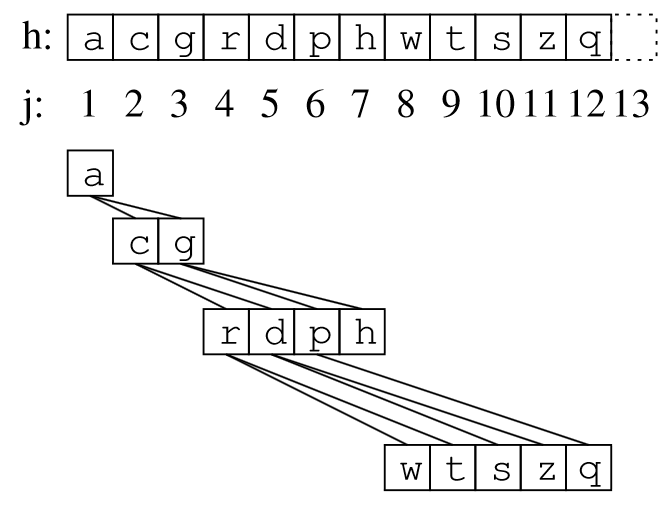
\includegraphics[height=4.7cm]{heaparray}
	\end{columns}
\end{frame}

\begin{frame}{Binäre Heaps}
	\begin{itemize}
		\item $insert$: Nach unten und \emph{siftUp}
		\item $deleteMin$: Element ganz unten rechts \~~> ganz oben, \emph{siftDown}
		\item $buildHeap$: „Ebenen“ von unten \~~> oben durchgehen und „down-siften“ \quad in $O(n)$
	\end{itemize}
\end{frame}





\begin{frame}{Sortierte Folgen -- (a, b)-Bäume}
	\textbf{Beispiel: (2, 4)-Baum} („00“ steht in VL für $\infty$) \\[0,125cm]
	\begin{figure}[htp]
		\centering
		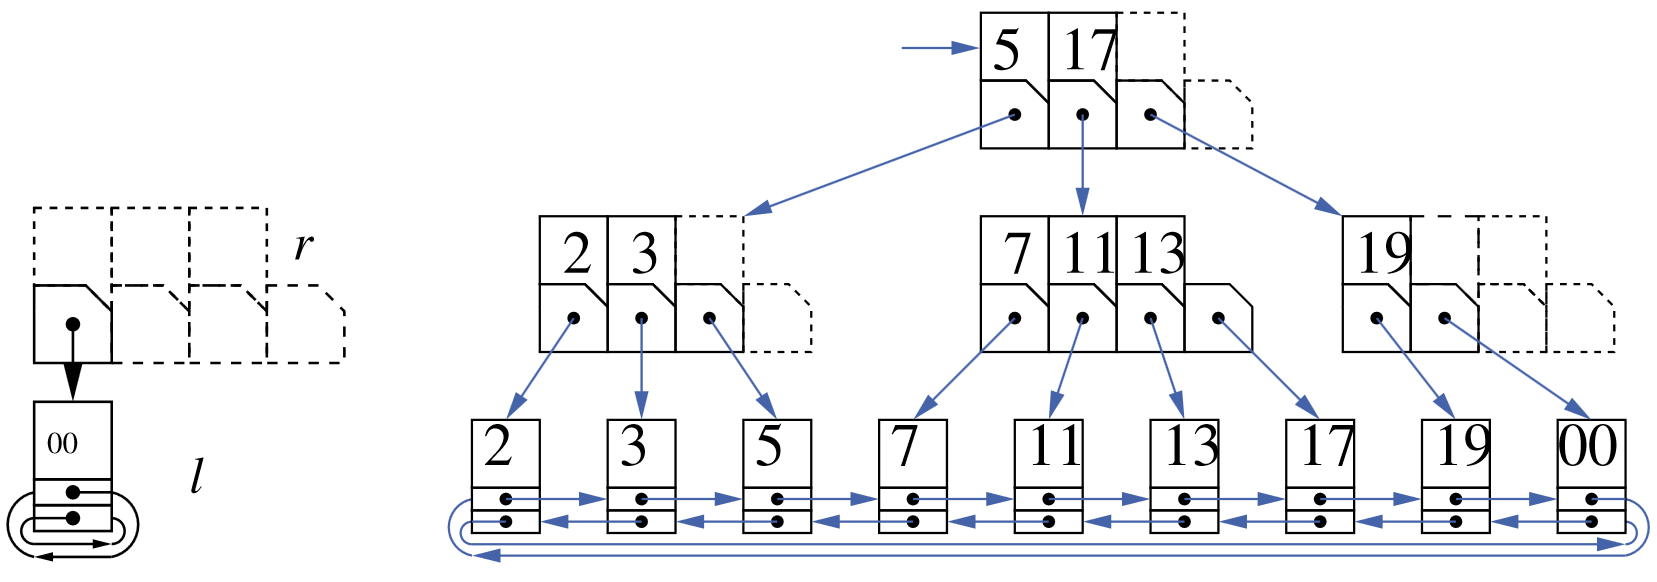
\includegraphics[width=\textwidth]{baum24}
	\end{figure}
\end{frame}




\begin{frame}{Graphen}
	\textbf{Repräsentationen} 
	\pause
	\begin{itemize}
		\item Kantenfolge
		\item Adjazenzmatrix
		\item Adjazenzfeld
		\item Adjazenzliste
	\end{itemize}
	
	\textbf{Durchlaufen}
	\begin{itemize}
		\item Tiefensuche
		\item Breitensuche
		\implitem Kantenklassifikation
	\end{itemize}
\end{frame}

\begin{frame}{Graphen}
	\textbf{Kürzeste Wege}
	\begin{description}
		\item[\textbf{Dijkstra}] Kantengewichte $\geq 0$, \quad $O((m+n) \log n)$
		\item[\quad\textbf{Bellman-Ford}] Kantengewichte $\in \R$, erkennt neg. Zyklen, \quad $O(n \cdot m)$
	\end{description}
	\pause
	\textbf{Minimale Spannbäume}
	\begin{itemize}
		\item \emph{Schnitteigenschaft}: \textbf{Leichteste} Kante in nem Schnitt: Nehmen!
		\item \emph{Kreiseigenschaft}: \textbf{Schwerste} Kante in nem Kreis: Raus!
		\implitem \emph{Jarník-Prim}: Dijkstra-ähnlich – Aufspannen
		\implitem \emph{Kruskal}: Kanten von leicht \~~> schwer hinzufügen, wenn's geht
	\end{itemize}
	\pause
	\textbf{UnionFind} (für Kruskal)
	\begin{itemize}
		\item Kleine Bäumchen repräsentieren \textbf{Knoten}mengen
		\item Pfadkompression
		\item Union-By-Rank
	\end{itemize}
\end{frame}



\begin{frame}{Optimierungsprobleme}
	\textbf{Ansätze:}
	\begin{itemize}
		\item Greedy
		\item DP
		\item[...] (s. VL)
		\item ILPs
	\end{itemize}
	\forcenewline
	{\small Aufgaben: 
		\begin{itemize}
			\item Altklausur März 2015 A3 „MaxSubArray“;
			\item Münzproblem (SS~2016 Übung~12 Folie~5 \\ {\footnotesize \url{http://crypto.iti.kit.edu/fileadmin/User/Lectures/Algorithmen\_SS16/ue12-slides.pdf}})
			\item Altklausur März 2017 A5 „Chemie-ILP“
		\end{itemize}
	}
\end{frame}



